\documentclass[]{extarticle}
\usepackage{comment}
\usepackage[hidelinks]{hyperref}
\usepackage{stackengine,xcolor}

\newcommand\shadowfy[1]{\expandafter\shadowfypars#1\par\relax\relax}
\long\def\shadowfypars#1\par#2\relax{%
  \ifx#1\relax\else
    \shadowfywords#1 \relax\relax%
  \fi%
  \ifx\relax#2\else\par\shadowfypars#2\relax\fi%
}
\def\shadowfywords#1 #2\relax{%
  \ifx#1\relax\else
    \shadowfyletters#1\relax\relax%
  \fi%
  \ifx\relax#2\else\ \shadowfywords#2\relax\fi%
}
\def\shadowfyletters#1#2\relax{%
  \shadow{#1}%
  \ifx\relax#2\else\shadowfyletters#2\relax\fi}

\newlength\shadowHoffset
\newlength\shadowVoffset
\setlength\shadowHoffset{.2pt}
\setlength\shadowVoffset{.1pt}
\def\primarycolor{white}
\def\secondarycolor{black}

\def\shadow#1{\setstackgap{L}{0pt}\def\stacktype{L}%
\def\useanchorwidth{T}% CAN BE COMMENTEDD FOR MORE INTERLETTER SPACE.
\Longstack{%
\raisebox{0pt}{\textcolor{\primarycolor}{#1}} 
\kern.7\shadowHoffset\raisebox{.7\shadowVoffset}{\textcolor{\secondarycolor}{#1}}
\kern-.7\shadowHoffset\raisebox{.7\shadowVoffset}{\textcolor{\secondarycolor}{#1}}
\kern\shadowHoffset\raisebox{0pt}{\textcolor{\secondarycolor}{#1}}
\kern-\shadowHoffset\raisebox{0pt}{\textcolor{\secondarycolor}{#1}}
\kern.7\shadowHoffset\raisebox{-.7\shadowVoffset}{\textcolor{\secondarycolor}{#1}}
\kern-.7\shadowHoffset\raisebox{-.7\shadowVoffset}{\textcolor{\secondarycolor}{#1}}
\kern0pt\raisebox{\shadowVoffset}{\textcolor{\secondarycolor}{#1}}
\kern0pt\raisebox{-\shadowVoffset}{\textcolor{\secondarycolor}{#1}}%
}}
\usepackage[paperheight=15in,paperwidth=15in,left=0.5in,right=0.5in,top=0in,bottom=0in]{geometry}
\usepackage{tikz}
\usepackage{fontspec}
\usepackage{polyglossia}
\setdefaultlanguage{french}
\setotherlanguages{english,russian}
\newfontfamily\footerfont[Path=./fonts/,SizeFeatures={Size=30}]{Tahoma}
\newfontfamily\cyrillicfont{Tahoma Bold}[Path=./fonts/,Script=Cyrillic]
\setmainfont{DejaVuSerif}[Path=./fonts/,Scale=MatchLowercase,NFSSFamily=french,Extension=.ttf,UprightFont={*},BoldFont={*-Bold},ItalicFont={*-Italic},BoldItalicFont={*-BoldItalic}]
\usepackage{xunicode}
\usepackage{xltxtra}
\pagestyle{empty}
\begin{document}
%
% Background
%
\begin{tikzpicture}[remember picture,overlay]
\node[inner sep=0] at (current page.center)
{\includegraphics[width=\paperwidth,height=\paperheight]{alacarte.png}};
\end{tikzpicture}
\def\primarycolor{orange!99}
\def\secondarycolor{black}
%
% Header
%
\begin{tikzpicture}[remember picture,overlay]
\node[inner sep=0,yshift=-0.5in,anchor=north] at (current page.north)
{\resizebox*{\textwidth}{!}{\shadowfy{კარგი მანერები}}};
\end{tikzpicture}
\begin{comment}
%
% Footer links
%
\begin{tikzpicture}[remember picture,overlay]
\node[inner sep=0,yshift=-6.6in,anchor=west] at (current page.center)
{
\includegraphics[width=31pt]{facebook.png}};
\node[inner sep=0,yshift=-7.1in,anchor=west] at (current page.center)
{
\includegraphics[width=31pt]{instagram.png}};
\node[inner sep=36pt,yshift=-6.6in,anchor=west] at (current page.center)
{\footerfont{\href{facebook.com/russianforthaisbyjibby}{facebook.com/russianforthaisbyjibby}}};
\node[inner sep=36pt,yshift=-7.1in,anchor=west] at (current page.center)
{\footerfont{\href{instagram.com/russianforthaisbyjibby}{instagram.com/russianforthaisbyjibby}}};
\end{comment}
%
% Content
%
\begin{tikzpicture}[remember picture,overlay]
\node[inner sep=0] at (current page.center)
{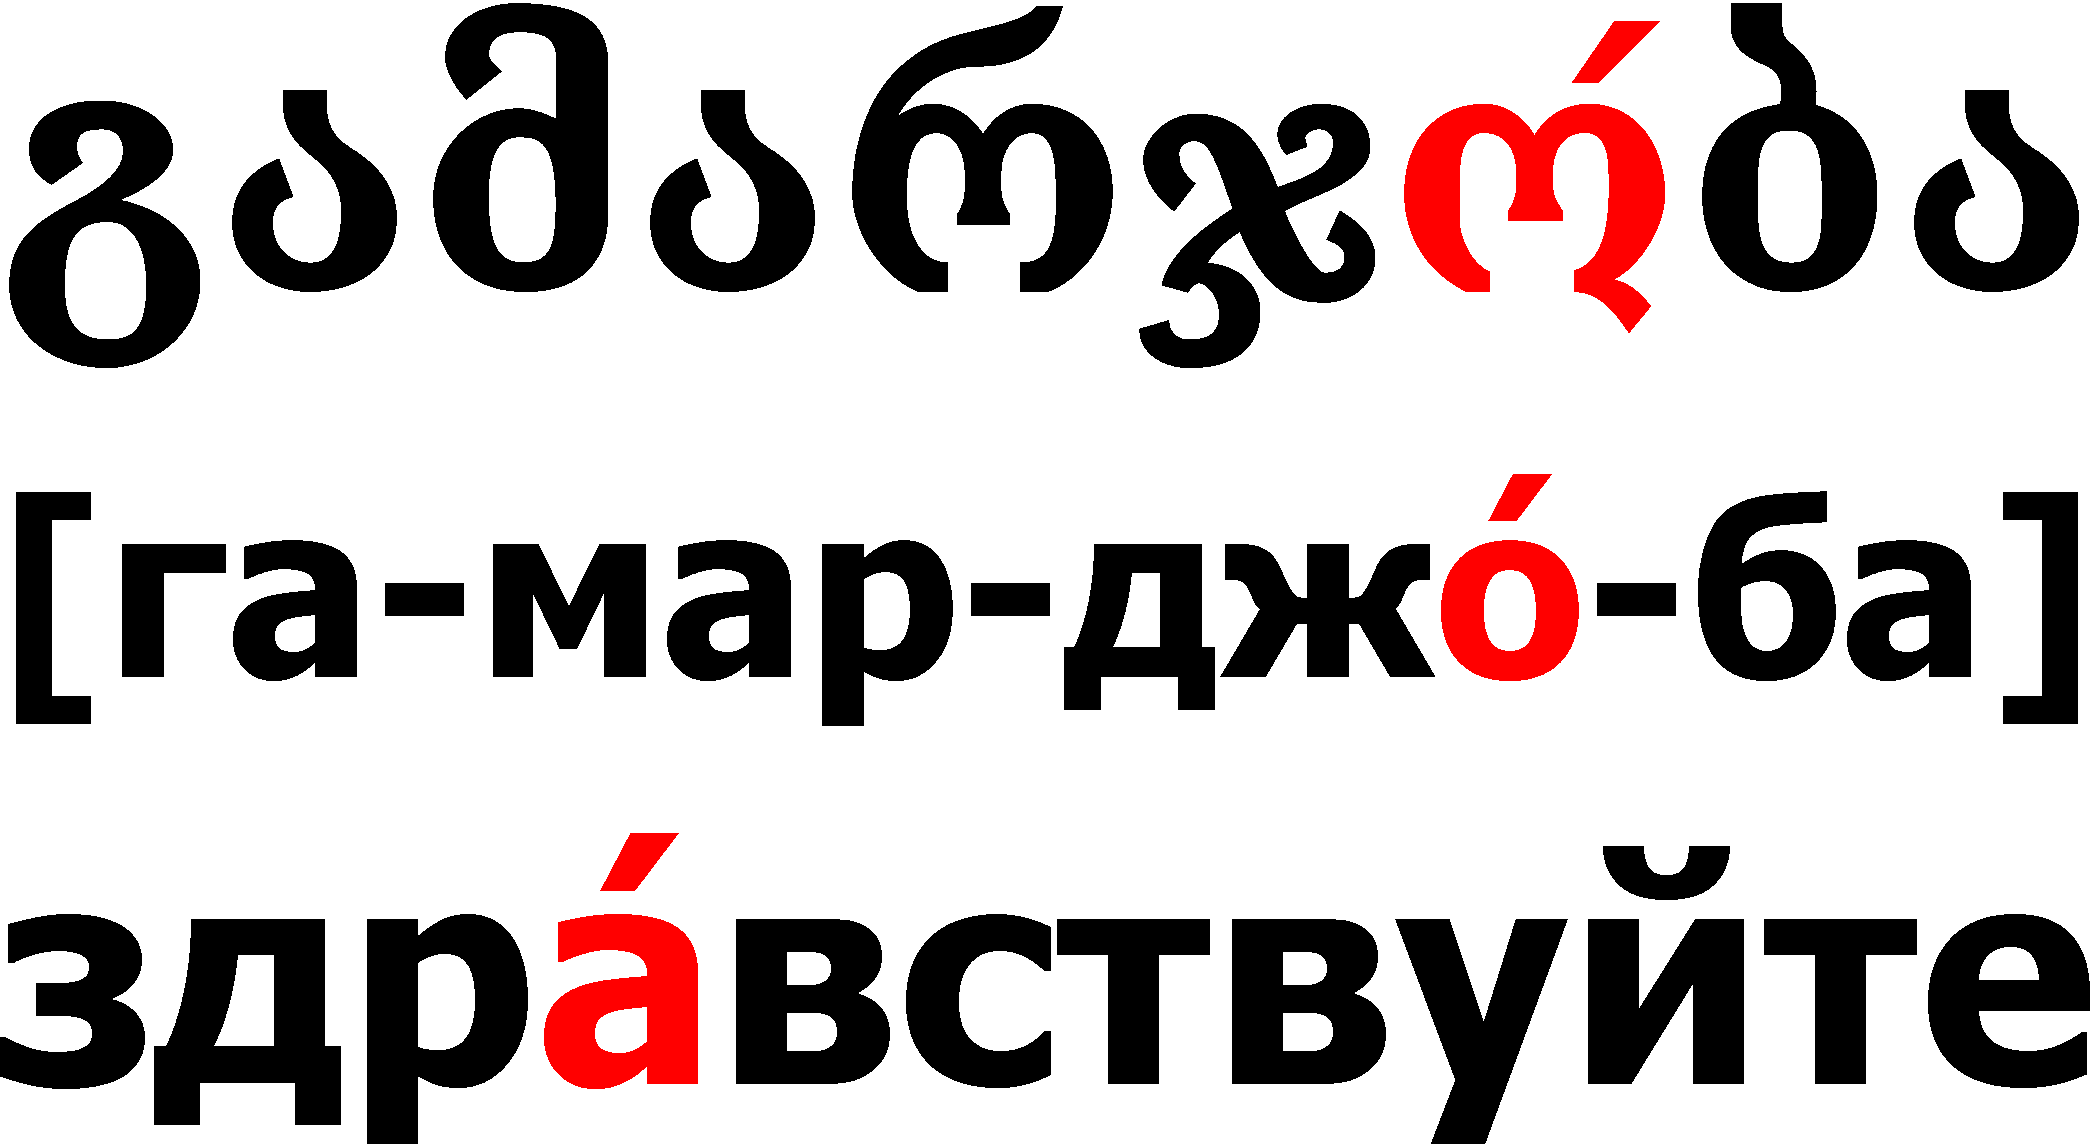
\includegraphics[width=0.9\paperwidth,height=0.8\paperheight,keepaspectratio]{content-crop.pdf}};
\end{tikzpicture}
\pagebreak
\end{document}
